%*********************************************************************
% 中国人民大学硕士毕业论文模板
% Copyright 2022 Ruoyang Guo, Pan Du
% 2020/06/06 v1.0 beta
%
%本文编写的依据是中国人民大学教务处2018年修订的《研究生毕业论文（设计）指导手册》
%本文的给出例子是在Qiu Renxiang本科毕业论文，Pan Du 硕士论文模版上进行改造。
%本文基本满足手册中对硕士论文的格式要求，并自动生成图表目录并编号，引用和目录也都具有超链接
% 重要提示：
%   1. 请确保使用 UTF-8 编码保存
%   2. 请使用 XeLaTeX编译
%   3. 修改、使用、发布本文档请务必遵循 LaTeX Project Public License
%   4. 不需要的注释可以尽情删除
%*********************************************************************
\documentclass[12pt,UTF8,twoside]{ctexart}

\usepackage{amsthm}
\newtheoremstyle{mystyle}{}{}{\upshape}{}{\bfseries}{:}{.5em}{}
\theoremstyle{mystyle}
\newtheorem{theorem}{定理}
\newtheorem{definition}{定义}
\newtheorem{property}{性质}
\newtheorem{lemma}{引理}

\usepackage{amsmath,amssymb,amsfonts}
\usepackage{algpseudocode}
\usepackage{float}
\usepackage{cite}
\usepackage{listings}
\usepackage{graphicx}
\usepackage{booktabs}
\usepackage{multirow}
\usepackage{geometry}
\usepackage{hyperref}
\usepackage{enumerate}
\usepackage{enumitem}
\usepackage{needspace}
\usepackage[section]{placeins}
\usepackage{threeparttable}
\usepackage{fancyhdr}
\usepackage{setspace}
%\usepackage{mathptmx}%Times New Roman字体
\usepackage{titletoc}
\usepackage{fontspec}
\setmainfont{Times New Roman}
\usepackage{pdfpages}
\usepackage{tikz}
\usepackage{etoolbox}
\usepackage{xcolor}
\usepackage{caption}
\usepackage{array}
\usepackage{tabularx}
\usepackage{titlesec}
%\usepackage{subfigure}
\usepackage{diagbox}
\usepackage{bbm}
%\usepackage{algorithm}
%\usepackage{algorithmicx}
% \usepackage{algorithmic}
% \usepackage{algorithm2e}
% \usepackage[ruled]{algorithm2e}                                     %算法排版样式1
% \usepackage[ruled,vlined]{algorithm2e}                          %算法排版样式2
% \usepackage[linesnumbered,boxed]{algorithm2e} 


%pam
\usepackage{bm}
\usepackage[ruled,linesnumbered]{algorithm2e}
\usepackage{subfig}
\usepackage{makecell}
\usepackage{bibspacing}
\newcommand{\fixdisplayspacing}{%
  \setlength{\abovedisplayskip}{1pt}%
  \setlength{\belowdisplayskip}{5pt}%
  \setlength{\abovedisplayshortskip}{1pt}%
  \setlength{\belowdisplayshortskip}{5pt}%
}
\setlength{\bibspacing}{0\baselineskip}
\setlist[enumerate]{itemsep=0pt,parsep=0pt,topsep=4pt,partopsep=0pt}
\setlist[itemize]{itemsep=0pt,parsep=0pt,topsep=4pt,partopsep=0pt}
\setlength{\parskip}{0pt}
\setlength{\emergencystretch}{2em}
\fixdisplayspacing
\makeatletter
\g@addto@macro\normalsize{\fixdisplayspacing}
\makeatother
\everydisplay{\fixdisplayspacing}
\setlength{\jot}{3pt}
\setlength{\textfloatsep}{8pt plus 2pt minus 2pt}
\setlength{\intextsep}{8pt plus 2pt minus 2pt}
\setlength{\floatsep}{8pt plus 2pt minus 2pt}
\AtBeginEnvironment{tabular}{\renewcommand{\arraystretch}{1.5}\setlength{\extrarowheight}{1pt}}
\AtBeginEnvironment{tabularx}{\renewcommand{\arraystretch}{1.5}\setlength{\extrarowheight}{1pt}}
% \BeforeBeginEnvironment{figure}{\par\Needspace{6\baselineskip}}
% \BeforeBeginEnvironment{table}{\par\Needspace{6\baselineskip}}

\usepackage{afterpage}
\newcommand\myemptypage{
    \null
    \thispagestyle{empty}
    \addtocounter{page}{-1}
    \newpage
    }
    
\newcommand{\eref}[1]{(\ref{#1})}
%pam


%图表目录重定义
%\renewcommand {\thetable} {\thesection{}.\arabic{table}}
%\renewcommand {\thefigure} {\thesection{}.\arabic{figure}}

\renewcommand {\thetable} {\thesection{}-\arabic{table}}
\renewcommand {\thefigure} {\thesection{}-\arabic{figure}}
\numberwithin{equation}{section}
\renewcommand {\theequation} {\thesection{}-\arabic{equation}}
\DeclareCaptionLabelSeparator{twospace}{\ ~}  
\captionsetup{labelsep=twospace,skip=6pt}


\renewcommand{\algorithmicrequire}{\textbf{输入:}}  
\renewcommand{\algorithmicensure}{\textbf{输出:}}  
\floatname{algorithm}{算法}


\renewcommand{\KwIn}{\textbf{输入:}}  
\renewcommand{\KwOut}{\textbf{输出:}}  
\renewcommand{\algorithmcfname}{算法}

%博士学生毕业论文要求纵向打印，页边距的要求为：
%上（T）：45mm
%下（B）：40mm
% 左（L）：35mm
% 右（R）：30mm
% 装订线（T）：0.5 cm
% 装订线位置（T）：左

\geometry{a4paper,left = 3.5cm,right = 3cm,top = 4.5cm,bottom = 4cm}


% 页眉：学校标志（教务处主页提供下载）：
% 高度为0.98 cm，宽度为4.13 cm，居中放置。
% 页码采用10.5号宋体字，居中放置，格式为：第1页。

\pagestyle{empty}
\lhead{}
\chead{}
\rhead{}
\lfoot{}
\rfoot{}

%目录和引用超链接
\hypersetup{
colorlinks=true,
linkcolor=black,
citecolor=black
}

\begin{document}
\raggedbottom

\newcommand\dunderline[3][-1pt]{{%
  \setbox0=\hbox{#3}
  \ooalign{\copy0\cr\rule[\dimexpr#1-#2\relax]{\wd0}{#2}}}}


%添加封面
\begin{titlepage}
  \vspace*{-10mm}
  \centering

  
\includegraphics[scale = 1.5]{figures/title.jpg}

  \vspace*{3mm}

  {\zihao{1}\heiti 专业硕士学位论文}

  \vspace*{3mm}
  {\zihao{5}\bfseries \mbox{THESIS OF PROFESSIONAL MASTER DEGREE}}
  \vspace{26mm}

  \zihao{1}\heiti

  \flushleft
  \begin{spacing}{1.3}
    \centering
    {\heiti\zihao{-2}\selectfont 论文题目：\dunderline[-10pt]{1pt}{\parbox[c]{112mm}{\centering 基于多模态数据的众筹结果预测研究}}\par}
    \vspace{4mm}

    {\heiti\zihao{-2}\selectfont （英\hspace{7mm}文）：\dunderline[-10pt]{1pt}{\parbox[b][18mm][c]{112mm}{\centering Research on Crowdfunding Outcome\\ Prediction Based on Multimodal Data}}\par}
    \vspace{4mm}

    {\heiti\zihao{-2}\selectfont 作\hspace{12mm}者：\dunderline[-10pt]{1pt}{\makebox[112mm][c]{周恋程}}\par}
    \vspace{4mm}

    {\heiti\zihao{-2}\selectfont 指导教师：\dunderline[-10pt]{1pt}{\makebox[112mm][c]{许伟}}\par}
    \vspace{4mm}

    {\heiti\zihao{-2}\selectfont 完成日期：\dunderline[-10pt]{1pt}{\makebox[112mm][c]{2026年3月12日}}\par}
  \end{spacing}

  \vspace{25mm}

\end{titlepage}


%%添加摘要
\input{textfiles/abstract}

% \myemptypage

%%添加目录
\newpage
\setcounter{page}{1}
\pagenumbering{arabic}
\pagestyle{fancy}
% \pagestyle{empty}
\lhead{}
\chead{}
\rhead{}
\lfoot{}
\rfoot{}
\fancyfoot[LO, RE]{}
\fancyfoot[OR, LE]{\footnotesize \thepage}
\setlength{\headheight}{14.5pt}
\setlength{\topskip}{0pt}
\renewcommand\contentsname{目\ 录}
\renewcommand\listfigurename{图\ 目\ 录}
\renewcommand\listtablename{表\ 目\ 录}
\tableofcontents
\newpage
\listoffigures
\listoftables
\newpage

% \myemptypage


% \fancyfoot[C]{\songti 第\thepage 页}
\setcounter{page}{1}
\pagenumbering{arabic}
\pagestyle{fancy}
\renewcommand{\headrulewidth}{.5pt}
\lhead{}
\chead{基于多模态数据的众筹结果预测研究}
\rhead{}
\lfoot{}
\rfoot{}
\fancyfoot[LO, RE]{}
\fancyfoot[OR, LE]{\footnotesize \thepage}
% \rfoot{\footnotesize \thepage }
% 按照自然段依次排列，每段起行空两格，回行顶格。12号宋体字，（重点文句，12号宋体字，加粗），倍行距20pt。
%正文、注释双面打印，编排页码，自第1页起，设置页眉。
%大标题(第1章)       黑体小二号（18pt），占六行（按宋体小四号计）居中
\titleformat{\section}[block]{\centering\heiti\LARGE\bfseries}{第\arabic{section}章}{1em}{}[]
\titlespacing{\section}{0pt}{27pt}{27pt}
%一级节标题（1.1）    黑体小三号（14pt），占四行（按宋体小四号计）顶头
\titleformat{\subsection}[block]{\heiti\Large}{\arabic{section}.\arabic{subsection}}{1em}{}[]
\titlespacing{\subsection}{0pt}{17pt}{17pt}
%二级节标题（1.1.1）  黑体小四号（12pt），占两行（按宋体小四号计）顶头
\titleformat{\subsubsection}[block]{\heiti\large}{\arabic{section}.\arabic{subsection}.\arabic{subsubsection}}{1em}{}[]
\titlespacing{\subsubsection}{0pt}{6pt}{6pt}
%倍间距20pt
\setlength{\baselineskip}{20pt}
\fixdisplayspacing

\input{textfiles/chapter1_introduction}
\newpage
\setcounter{table}{0}
\setcounter{figure}{0}
\section{相关文献综述}
\subsection{众筹结果影响因素研究}
本次研究的研究对象为基于奖励的众筹市场，在该市场环境下，投资者与项目方信息不对称的现象普遍存在，因此项目方披露的信息对众筹结果至关重要，投资者往往基于此进行决策。现已有大量研究从实证角度探讨项目成功的影响因素，主要涵盖项目元信息、文本内容、视觉呈现与项目互动等维度。这些研究不仅揭示了众筹结果的内在影响因素，也为预测模型中的特征选择提供了理论指导。

在以往的研究范式中，众筹页面通常被抽象为一组高维的特征向量，通过统计学检验或机器学习方法建立变量与众筹结果之间的关联。

从项目主体视角出发，项目目标金额、发起时间、项目类别等元信息在绝大多数研究中被广泛使用，在众筹绩效预测模型中发挥着基础性作用。除上述基础信息之外，既有研究多关注发起人社交资本、动态行为及历史经验对众筹结果的影响。例如，Kao 等研究了发起人之间的社交网络对项目投入产出比的影响，实证结果表明，项目发起人之间通过互惠和联结积累的社交资本显著优化了项目从资源投入到资金产出的转化过程\cite{ref16}；互动的即时性与深度也是研究热点，李清香等研究发现，发起人与出资者之间的双向在线互动显著影响众筹结果，其中出资者评论的情感倾向以及发起人回复的长度均与筹资成功率正向相关\cite{ref17}；在经验积累维度，王念新等的研究表明，项目发起人通过过往发起项目和支持他人项目所积累的直接或间接经验显著提升了项目成功率\cite{ref18}。

在项目主体信息之外，随着多媒体技术在平台中的普及，多模态信息在影响众筹结果中也发挥关键作用。既有研究表明，多模态元素的丰富度与内容质量显著影响融资绩效。例如，Carradini 等研究发现，成功的众筹项目往往比失败项目使用了更多的图片、视频等非文本元素，在内容表现上具有明显优势，形成了更强的感官冲击\cite{ref19}；Raab 等考察了图片中显示的面部情绪表达如何影响资助决策，发现快乐和悲伤的面部表情能够引发共情，对投资者的资助决策有正向诱导作用\cite{ref20}；Costello 等探讨了众筹中文本模糊性和双面性对项目融资成功可能性的影响，强调了表述清晰度在建立契约信任中的重要性\cite{ref21}；封面图作为项目的第一视觉入口具有特殊影响力，Chen 等研究了在众筹平台上封面图像如何影响资助结果，以及对于不同类型的众筹活动影响有何不同\cite{ref22}。尽管这些多模态特征在解释性研究中日益受到重视，但它们很少被系统纳入预测模型的特征工程或深度学习框架中，这构成了本研究后续开展多模态融合预测研究的重要切入点。

\subsection{众筹领域中的多模态预测研究}
鉴于影响众筹结果的因素众多，且呈现出多模态并存的特征，过往预测研究已从单一模态逐步转向复杂的多模态融合范式。

早期研究多聚焦于单一模态。在文本侧，研究者在预测模型中加入项目描述、项目评论等文本信息，以提升模型的预测效果：Song 等使用 RWW 框架分析文本，建立了技术类众筹的预测模型\cite{ref23}；Bao 等提出了从评论中挖掘语义特征的新框架，以改进筹款成功预测\cite{ref24}。在视觉侧，视觉信息（图片、视频）对于吸引潜在支持者、传达项目理念、展示产品特性以及激发捐款意愿有着直接的影响，因此 Blanchard 等重点关注了视觉特征的提取，并使用机器学习方法预测众筹项目筹集到的总金额\cite{ref25}。

近年来，使用多模态模型整合多维信息进行众筹结果预测成为了主流方向。其中，Cheng 等提出的多模态深度学习（MDL）模型是该领域的开创性工作之一\cite{ref12}。该研究首次将视觉图像作为除文本和元数据之外的重要模态引入众筹预测任务中，设计了三个并行分支：顶部分支利用 One-hot 编码处理类别和筹资目标等元数据；中间分支利用预训练的 VGG16 网络提取项目描述中多张图像的深层特征；底部分支则通过词嵌入对文本进行语义编码。模型最终通过全连接层实现各模态特征的晚期融合，实验证明引入视觉信息能显著提升预测准确率，特别是在文本信息匮乏的项目中表现优异。


\begin{figure}[H]
  \centering
  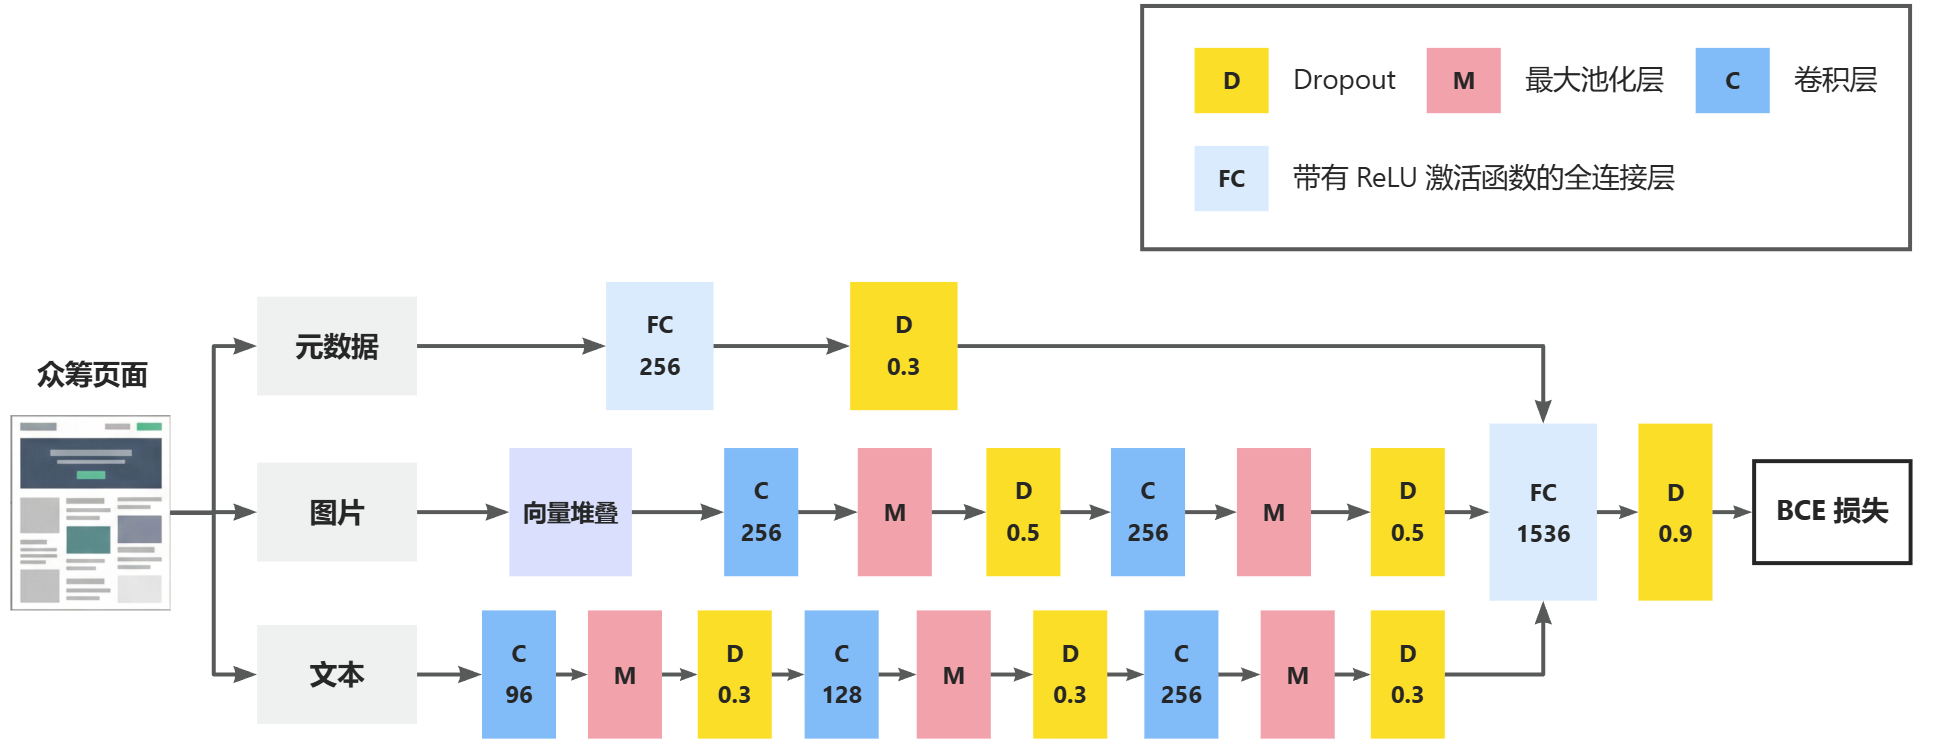
\includegraphics[width=0.95\textwidth]{figures/MDL.jpg}
  \caption{MDL模型结构参数图（重绘自论文\cite{ref12}）}
  \label{fig:mdl_13}
\end{figure}

在 MDL 奠定的基础上，后续研究开始探索更精细的特征工程与多模态融合策略。Kaminski 利用文本、语音、视频元数据构建预测模型，强调语言风格与可视化演示的重要性\cite{ref11}；徐琳整合了数值、文本和图像三种模态，并采用证据理论融合模型进行决策预测\cite{ref26}；Al-Qershi 等深入挖掘了众筹广告中的哪些内容特征更有助于准确预测众筹成功，设计了 1368 个细粒度特征，并使用集成学习模型提升了预测的适应性\cite{ref27}。

最新研究在视频模态的引入和模态交互的深度上取得了进一步突破。Tang 等针对众筹页面中信息含量极高的介绍视频，提出了深度交叉注意力网络（DCAN），该模型创新性地开发了跨模态交叉注意力块（Cross\hspace{0pt}-\hspace{0pt}Attention\hspace{0pt} Block）来对齐文本描述与长视频，在有效缓解数据噪声的同时提升了跨模态交互质量\cite{ref13}。Zhang 和 Lau 结合项目描述文本、音频片段和视频片段等多模态特征，通过将音视频信号转录为文本并进行晚期融合，证明了多模态协同较单一模态具有显著优势\cite{ref28}。Cai 等提出了多模态动态图卷积网络（MDGCN），将多模态交互建模提升到了图结构层面，增强了模型捕获复杂模态关联的能力\cite{ref14}。Li 等针对众筹场景下模态间语义关联较弱的挑战，提出了共性增强的多模态解耦框架（CAMD），通过将异构数据映射至模态不变空间与模态特定空间，并利用增强网络放大潜在的跨模态共性，实现了更为平衡且稳健的特征表示\cite{ref15}。

上述研究共同推动了众筹预测从单一模态分析向复杂多模态深度交互的范式演进，极大地提升了模型的特征表征能力。然而，尽管现有模型探讨了更复杂的多模态交互结构，但仍主要关注模态内容本身的语义信息，缺乏对内容呈现方式的建模。这些方法往往把文本、图片、视频内容视为语义信息的集合，却忽略了众筹界面图文依序排布所形成的叙事逻辑，以及排版的视觉密度对潜在投资者认知负荷的影响。鉴于此，本研究通过 Transformer 架构捕捉图文交替中的叙事节奏与视觉密度特征，旨在从众筹界面的内容呈现结构这一新视角提升众筹结果预测的准确度。

\subsection{多模态内容呈现理论}
众筹项目的页面浏览本质上是一个高强度的信息摄取与决策过程。出资人在面对陌生项目时，既需处理项目本身的内在复杂性，又需、应对信息呈现方式所带来的外在认知负荷。因此，项目描述区的内容呈现直接决定了信息的传递效率与用户的决策行为。

首先，视觉密度深刻影响着用户的阅读意愿。视觉密度是指在给定界面空间内信息元素（包括文本、图像、图标及装饰性元素）的集中程度。认知负荷理论指出，人类的工作记忆容量有限，视觉密度的管理本质上是对用户有限的注意力资源进行调度。如果多模态界面视觉密度过高，单位面积内的信息量（如字数、图片）超出了工作记忆的承载范围，就会引发认知过载与逃离行为\cite{ref29,ref30,ref31}。Djamasbi 等的眼动追踪研究进一步证实，Web 用户倾向于 F 型扫描，高密度文本会导致视线在垂直扫描中滑落\cite{ref32}。Liang 等的研究也证明，在文本维度上，众筹项目的字数与融资成功率之间存在显著的“倒 U 型”关系\cite{ref33}。字数一旦超过某个特定阈值，过剩的信息就会转化为外在负荷，形成理解负担，反而降低了投资者的支持意愿。在此基础上，加工流畅性理论进一步解释了这一现象\cite{ref34}：文本长度、图片大小等视觉密度特征直接影响界面认知负荷，当页面呈现出较低的认知负荷时，投资者会产生更高的加工流畅性，这种轻松的心理感受往往会转化为对项目质量的直觉判断，进而提升投资意愿。这意味着众筹项目界面不应追求极端的信息堆砌，而应通过优化视觉密度来匹配投资者的认知能力。

除视觉密度等静态属性外，图文内容的排列顺序同样是决定说服效果的关键变量。研究表明，人类对信息的加工具有显著的顺序依赖性。根据 Hogarth 和 Einhorn 提出的信念修正模型\cite{ref35}，个体在接收序列信息时，会以当前信念为锚点，并根据后续信息进行调整和加权。在这种序贯加工过程中，信息的呈现顺序会直接改变权重的分配，导致相同的多模态刺激产生截然不同的判断结果。在 Web 环境下，用户往往采取自上而下顺序浏览的信息处理模式，使得符合阅读习惯的“倒金字塔”结构及图文交替的呈现节奏能够通过优化认知路径来增强内容说服力\cite{ref36}。这种顺序效应在多个领域得到了实证：在新闻领域，Tjärnhage 等发现交互式图文叙事能有效维持用户注意力\cite{ref37}；在电商领域，Lee 等发现图片的排列顺序会影响消费者的购买意愿\cite{ref38,ref39}；在广告领域，Razak 等指出文字和视觉元素共同构成了广告的说服过程，广告往往优先使用具有吸引力的图片抓取消费者注意力，随后再使用文字通过深入的信息披露来完成说服\cite{ref40}。因此，在以 Kickstarter 为代表的众筹场景中，图文顺序所蕴含的叙事结构也不仅仅是信息披露的载体，更是决定筹资说服力的核心逻辑。

从深层心理机制看，视觉密度和排列顺序对众筹成功性的影响可以用叙事传输理论来解释：该理论指出，受众能否被叙事带入情境并产生信念偏转，高度依赖于叙事质量\cite{ref41}。在众筹的多模态情境下，叙事质量具体转化为两个维度：顺序决定了叙事的方向感与逻辑自洽性，而视觉密度决定了叙事的呼吸感与情绪节奏，二者共同决定了项目内容对潜在支持者的说服效果。本研究对众筹项目的内容呈现方式进行建模，旨在量化项目的“叙事传输”对众筹成功性的影响。

\subsection{内容呈现结构建模的工程实践}
鉴于内容呈现结构的重要性，多模态深度学习模型在行为预测领域已形成了较为成熟的工程化建模方案。以微软 LayoutLM 系列模型为代表的系列工作，开创性地将文本、布局坐标和视觉信息统一到同一个预训练框架中，奠定了多模态布局建模的基础\cite{ref42,ref43}。这种布局信息的效用在多个交互场景中得到了实证：在点击率预测领域，Cui 等提出了基于扩散模型的多模态协同兴趣网络，通过建模图文在特定布局下的复杂交互与协同效应，证实了捕捉模态间的空间关联对于提升点击率预测精度的关键作用\cite{ref44}；在新闻推荐领域，Chai 等发现“左图右文”的排列方式更符合人类的认知加工习惯，证实了图文出现的物理顺序与空间占位会直接干预用户的认知效率\cite{ref47}。上述研究均表明，引入布局信息是提升模型预测精度的重要途径。

这种建模趋势的背后有着深层的认知与方法论支撑。Paivio 提出的双重编码理论指出，大脑在处理图文交替信息时，文字和视觉信息是由不同系统并行加工但又相互关联的\cite{ref45}。然而，在传统深度学习中，这种多模态特征往往因模态不同、特征空间割裂而难以整合。CLIP 等预训练模型的出现，通过对比学习将不同模态映射至统一的表征空间，为双重编码理论提供了工程视角的模态间关联处理，已成为当前多模态融合的主流范式\cite{ref46}。其核心价值在于通过跨模态语义对齐，使模型能够超越单纯的特征堆砌，转而捕捉图文序列中深层的叙事逻辑。

由此审视众筹场景，虽然其页面不像复杂文档那样具有多变的二维布局，但其图文叙事序列实质上构成了特定场景下一种线性的、流式的布局结构。这种结构虽然在空间维度上进行了简化，但在逻辑维度上对众筹绩效的影响依然存在。然而，现有众筹研究大多关注模态具体内容，鲜有研究系统量化这种图文布局模式对融资绩效的影响。本研究旨在填补这一空白，将上述对内容呈现结构的建模思想引入众筹领域，对众筹项目描述页面的图文序列进行建模与分析。

\subsection{本章小结}
本章从众筹结果影响因素、预测模型、内容呈现理论及工程实践四个维度，对众筹领域的既有研究进行了全面回顾。

在影响因素层面，既有研究表明，奖励类众筹的结果受项目元属性（如目标金额、类别）、发起人社交资本等项目主体信息的影响。此外，随着多媒体内容的普及，已有大量研究证实图片、视频及文本等多模态因素在感官冲击与信任建立中发挥了重要作用。

基于对影响因素的研究，多模态众筹预测技术已实现从单一模态分析向深度多模态融合的转型。近期研究通过引入交叉注意力机制、图卷积网络及模态解耦框架，不断提升了模型对多模态数据的表征能力。然而现有研究大多关注内容语义本身，尚未对多模态内容的呈现方式进行建模。

为探讨多模态内容呈现方式影响众筹结果的机理，本章引入了认知负荷理论、加工流畅性理论及叙事传输理论在界面浏览中的应用。研究发现，过高的视觉密度会导致阅读者认知过载，而符合认知规律的线性叙事顺序则能优化权重的分配并增强内容的说服力。这为本研究进行叙事逻辑和视觉密度的量化提供了理论依据。

最后，本章调研了目前内容呈现结构建模的工程化实践方案。借鉴 LayoutLM 与 CLIP 等领先的布局建模与多模态预训练范式，建模众筹界面的内容呈现结构具有工程上的可行性，且该部分仍是现有众筹研究中鲜少被提及的切入点。

通过对相关文献的总结发现，虽然现有模型在多模态特征提取上取得了显著突破，但仍普遍忽略了众筹页面中图文编排的叙事逻辑与排版的视觉节奏。这正是后续章节开展内容呈现结构建模研究的核心动因。

\input{textfiles/chapter3_model_construction}
\input{textfiles/chapter4_experiments_and_analysis}
\input{textfiles/chapter5_conclusion}

\newpage
\addcontentsline{toc}{section}{参考文献}
\begin{thebibliography}{99}
\bibitem{ref1} Mitra T, Gilbert E. The language that gets people to give: Phrases that predict success on Kickstarter[C]//Proceedings of the 17th ACM Conference on Computer Supported Cooperative Work \& Social Computing. 2014: 49-61.
\bibitem{ref2} Yuan H, Lau R Y K, Xu W. The determinants of crowdfunding success: A semantic text analytics approach[J]. Decision Support Systems, 2016, 91: 67-76.
\bibitem{ref3} Popescul D, Radu L D, P\u{a}v\u{a}loaia V D, et al. Psychological determinants of investor motivation in social media-based crowdfunding projects: A systematic review[J]. Frontiers in Psychology, 2020, 11: 588121.
\bibitem{ref4} Mollick E. The dynamics of crowdfunding: An exploratory study[J]. Journal of Business Venturing, 2014, 29(1): 1-16.
\bibitem{ref5} Pekar V, Candi M, Beltagui A, et al. Explainable text-based features in predictive models of crowdfunding campaigns[J]. Annals of Operations Research, 2025, 354(1): 367-397.
\bibitem{ref6} Ardakani S P, Hu J, Zhang J, et al. Identifying crowdfunding storytellers who deliver successful projects: A machine learning approach[J]. The Journal of Supercomputing, 2025, 81(1): 263.
\bibitem{ref7} Zhang X, Lyu H, Luo J. What contributes to a crowdfunding campaign's success? Evidence and analyses from GoFundMe data[J]. Journal of Social Computing, 2021, 2(2): 183-192.
\bibitem{ref8} Zhang X, Zheng X, Luo J. The influence of stereotypes and visual features on donation intentions in online medical crowdfunding campaigns: A comparison of survey and large language model-based methods[J]. npj Artificial Intelligence, 2025, 1(1): 16.
\bibitem{ref9} 张卫国, 黄思颖, 王超. 奖励众筹融资绩效动态预测研究——来自“众筹网”数据的实证[J]. 中国管理科学, 2023, 31(5): 71-83.
\bibitem{ref10} 张凯, 赵洪科, 刘淇, 等. 基于动静态表征的众筹协同预测方法[J]. 软件学报, 2020, 31(4): 967-980.
\bibitem{ref11} Greenberg M D, Pardo B, Hariharan K, et al. Crowdfunding support tools: Predicting success \& failure[C]//CHI '13 Extended Abstracts on Human Factors in Computing Systems. 2013: 1815-1820.
\bibitem{ref12} Li Y, Rakesh V, Reddy C K. Project success prediction in crowdfunding environments[C]//Proceedings of the Ninth ACM International Conference on Web Search and Data Mining. 2016: 247-256.
\bibitem{ref13} Kaminski J C, Hopp C. Predicting outcomes in crowdfunding campaigns with textual, visual, and linguistic signals[J]. Small Business Economics, 2020, 55(3): 627-649.
\bibitem{ref14} Cheng C, Tan F, Hou X, et al. Success prediction on crowdfunding with multimodal deep learning[C]//Proceedings of the 28th International Joint Conference on Artificial Intelligence. 2019: 2158-2164.
\bibitem{ref15} Tang Z, Yang Y, Li W, et al. Deep cross-attention network for crowdfunding success prediction[J]. IEEE Transactions on Multimedia, 2022, 25: 1306-1319.
\bibitem{ref16} Cai Z, Ding H, Xu M, et al. Multimodal dynamic graph convolutional network for crowdfunding success prediction[J]. Applied Soft Computing, 2024, 154: 111313.
\bibitem{ref17} Li J, Xu X, Li Y, et al. Commonality augmented disentanglement for multimodal crowdfunding success prediction[C]//Proceedings of the 2025 IEEE International Conference on Acoustics, Speech and Signal Processing. 2025: 1-5.
\bibitem{ref18} 黄健青, 黄晓凤, 殷国鹏. 众筹项目融资成功的影响因素及预测模型研究[J]. 中国软科学, 2017(7): 91-100.
\bibitem{ref19} 李小倩, 赵文红, 吕斯尧, 等. 产品价值线索对众筹融资绩效的影响——创业者线索的调节作用[J]. 研究与发展管理, 2024, 36(2): 125-138.
\bibitem{ref20} Kao T W, Hsiao S H, Su H C, et al. Deriving execution effectiveness of crowdfunding projects from the fundraiser network[J]. Journal of Management Information Systems, 2022, 39(1): 276-301.
\bibitem{ref21} 李清香, 王念新, 吕爽, 等. 发起人与出资者的在线交互对众筹项目成功的影响[J]. 管理工程学报, 2020, 34(1): 118-126.
\bibitem{ref22} 王念新, 吕爽, 周园, 等. 连续发起人的经验对众筹成功的影响: 经验相关性的调节效应分析[J]. 管理工程学报, 2020, 34(4): 89-100.
\bibitem{ref23} Carradini S, Fleischmann C. The effects of multimodal elements on success in Kickstarter crowdfunding campaigns[J]. Journal of Business and Technical Communication, 2023, 37(1): 1-27.
\bibitem{ref24} Raab M, Schlauderer S, Overhage S, et al. More than a feeling: Investigating the contagious effect of facial emotional expressions on investment decisions in reward-based crowdfunding[J]. Decision Support Systems, 2020, 135: 113326.
\bibitem{ref25} Costello F J, Lee K C. Exploring investors' expectancies and its impact on project funding success likelihood in crowdfunding by using text analytics and Bayesian networks[J]. Decision Support Systems, 2022, 154: 113695.
\bibitem{ref26} 刘畅, 陈守明. 文本信息含量与公益众筹绩效研究——基于有限注意的视角[J]. 投资研究, 2022, 41(6): 96-113.
\bibitem{ref27} Chen S, Wang H, Fang Y, et al. Informational and emotional appeals of cover image in crowdfunding platforms and the moderating role of campaign outputs[J]. Decision Support Systems, 2023, 171: 113975.
\bibitem{ref28} Song C, Luo J, H\"oltt\"a-Otto K, et al. Crowdfunding for design innovation: Prediction model with critical factors[J]. IEEE Transactions on Engineering Management, 2020, 69(4): 1565-1576.
\bibitem{ref29} Bao L, Wang Z, Zhao H. Who said what: Mining semantic features for success prediction in reward-based crowdfunding[J]. Electronic Commerce Research and Applications, 2022, 53: 101156.
\bibitem{ref30} Blanchard S J, Noseworthy T J, Pancer E, et al. Extraction of visual information to predict crowdfunding success[J]. Production and Operations Management, 2023, 32(12): 4172-4189.
\bibitem{ref31} 徐琳. 多模态数据驱动的众筹项目成功率预测研究[D]. 合肥工业大学, 2022.
\bibitem{ref32} Al-Qershi O M, Kwon J, Zhao S, et al. Predicting crowdfunding success with visuals and speech in video ads and text ads[J]. European Journal of Marketing, 2022, 56(6): 1610-1649.
\bibitem{ref33} Zhang Z, Lau R Y K. Exploiting multimodal features and deep learning for predicting crowdfunding successes[C]//Proceedings of the 2024 IEEE International Conference on Omni-layer Intelligent Systems. 2024: 1-6.
\bibitem{ref34} Sweller J. Cognitive load theory[M]//Psychology of Learning and Motivation. Academic Press, 2011, 55: 37-76.
\bibitem{ref35} 何旭, 郭春彦. 视觉工作记忆的容量与资源分配[J]. 心理科学进展, 2013, 21(10): 1741-1748.
\bibitem{ref36} 车敬上, 孙海龙, 肖晨洁, 等. 为什么信息超载损害决策? 基于有限认知资源的解释[J]. 心理科学进展, 2019, 27(10): 1758-1768.
\bibitem{ref37} Djamasbi S, Siegel M, Tullis T. Visual hierarchy and viewing behavior: An eye tracking study[C]//Human-Computer Interaction: Design and Development Approaches. 2011: 331-340.
\bibitem{ref38} Liang X, Hu X, Jiang J. Research on the effects of information description on crowdfunding success within a sustainable economy—the perspective of information communication[J]. Sustainability, 2020, 12(2): 650.
\bibitem{ref39} Alter A L, Oppenheimer D M. Uniting the tribes of fluency to form a metacognitive nation[J]. Personality and Social Psychology Review, 2009, 13(3): 219-235.
\bibitem{ref40} Hogarth R M, Einhorn H J. Order effects in belief updating: The belief-adjustment model[J]. Cognitive Psychology, 1992, 24(1): 1-55.
\bibitem{ref41} Joshi A, Mathur G. The inverted pyramid approach in user interface design for interactive information retrieval[C]//Proceedings of the EASY3 (CHI South India) Annual Conference. 2004.
\bibitem{ref42} Tjärnhage A, Söderström U, Norberg O, et al. The impact of scrollytelling on the reading experience of long-form journalism[C]//Proceedings of the European Conference on Cognitive Ergonomics 2023. 2023: 1-9.
\bibitem{ref43} Lee J E, Shin E, Kincade D H. The effects of presentation order of apparel product images on consumers' information processing style and purchase intentions[C]//Proceedings of the International Textile and Apparel Association Annual Conference. 2019, 76(1).
\bibitem{ref44} Lee J E, Shin E, Kincade D H. Presentation-order effect of product images on consumers' evaluations in online shopping[C]//Proceedings of the International Textile and Apparel Association Annual Conference. 2020, 77(1).
\bibitem{ref45} Razak N A, Asma'Amran S N. Effective language use in advertising in the most visible online stores: 2 Case Studies[J]. International Journal of Education and Learning Systems, 2017, 2: 30-38.
\bibitem{ref46} Green M C, Brock T C. The role of transportation in the persuasiveness of public narratives[J]. Journal of Personality and Social Psychology, 2000, 79(5): 701-721.
\bibitem{ref47} Xu Y, Li M, Cui L, et al. LayoutLM: Pre-training of text and layout for document image understanding[C]//Proceedings of the 26th ACM SIGKDD International Conference on Knowledge Discovery \& Data Mining. 2020: 1192-1200.
\bibitem{ref48} Xu Y, Xu Y, Lv T, et al. LayoutLMv2: Multi-modal pre-training for visually-rich document understanding[C]//Proceedings of the 59th Annual Meeting of the Association for Computational Linguistics and the 11th International Joint Conference on Natural Language Processing. 2021: 2579-2591.
\bibitem{ref49} Cui X, Lu W, Tong Y, et al. Diffusion-based multi-modal synergy interest network for click-through rate prediction[C]//Proceedings of the 48th International ACM SIGIR Conference on Research and Development in Information Retrieval. 2025: 581-591.
\bibitem{ref50} Chai S, Chang Y, Li Y. Image-left, text-right: The horizontal sequence effect of images and text on consumer responses to in-feed news[J]. Psychology \& Marketing, 2025, 42(8): 2121-2135.
\bibitem{ref51} Paivio A. Mental representations: A dual coding approach[M]. Oxford University Press, 1990.
\bibitem{ref52} Radford A, Kim J W, Hallacy C, et al. Learning transferable visual models from natural language supervision[C]//Proceedings of the 38th International Conference on Machine Learning. 2021: 8748-8763.
\end{thebibliography}


\newpage
\addcontentsline{toc}{section}{致谢}
\section*{致谢}
又是一年毕业季，只是今年毕业的主角变成了我自己。在硕士生涯即将画上句号之际，我想对所有帮助过我的人致以最真诚的感谢。

首先，特别感谢我的导师许伟教授。感谢许老师一直以来对我的栽培，从大四那年提前带我进入课题组学习，到如今指导我完成硕士毕业论文，这几年的学术引导让我受益终身。在毕业论文撰写过程中，许老师每一次耐心的辅导与思路的点拨，总能让我豁然开朗。人们常说良师是智慧的灯塔，谢谢您一直以来的教诲，祝愿您身体健康，家庭幸福，工作顺利！

其次，我要感谢一直以来支持着我的家人。感谢我的家人，没有你们在背后的坚定支持，就不会有我今天的小小成就。如今我即将真正踏入社会，身上又多了一份作为成年人的责任，希望在不久的未来，我也能拥有保护和支持你们的力量。

同时，也感谢这两年来在中国人民大学结识的同门与朋友们。尤其感谢指导我进行众筹相关科研的杨少辰师兄。在论文撰写及模型调试过程中，师兄总是不吝赐教，耐心与我讨论并分享经验，让这篇论文得以更加严谨地呈现。尽管硕士生活只有匆匆两年，但与你们在校园里的交流与共处，构成了我生命中极为珍贵的记忆。此后天南海北，愿大家都能在各自的领域熠熠生辉。

最后，感谢中国人民大学给予我的培养。尽管即将告别校园走向新的岗位，但人大带给我的眼界、底气与情怀将伴随我一生。旧章落幕，新篇开启。祝愿母校年华常青，更上一层楼！

\end{document}

